\section{Results}

\subsection{ECG FMs have distinct depth--scale decomposition surfaces}

Figure~\ref{fig:semantic-atlas} summarizes single-coordinate clinical accessibility at three resolutions: test depth--scale surfaces for every FM, paired patient-bootstrap common-scale semantic AUCs, and concept-family profiles. The corresponding reconstruction and dead-feature atlases are included in Appendix~\ref{app:additional-atlases}. These surfaces are the primary result object: a model can localize clinical measurements more strongly at one depth while requiring a wider dictionary or exhibiting less stable atom identity elsewhere. We therefore retain all 25 depth--scale cells per model as the prespecified multiscale evaluation surface.

Interpretability is consequently represented as a structured profile of sparse reconstructability, single-coordinate clinical accessibility, coverage, and feature reproducibility. Common-scale AUC provides a capacity-robust comparison within each axis, while the underlying depth--scale surfaces support operating-point selection for specific analysis goals.

\subsection{Matched-scale curves produce metric-specific FM orderings}

Figure~\ref{fig:matched-curves} compares all FMs only at the same $E$. Shaded regions are paired patient-cluster intervals after averaging the three fixed SAE seeds and five target depths. For reconstruction, the highest common-scale point estimate is \MSReconTopModel{} (AUC \MSReconTopAUC{}, 95\% CI [\MSReconTopCILow{}, \MSReconTopCIHigh{}], bootstrap rank-1 probability \MSReconTopRankOne{}). The complete reconstruction order is \MSReconOrder{}, with \MSReconSignificantPairs{} of 15 pairwise contrasts surviving BH correction.

Single-coordinate clinical accessibility has a separate ordering: \MSSemanticOrder{}, with \MSSemanticSignificantPairs{} of 15 FM contrasts surviving BH correction. The matched model-level profile is complemented by substantial concept-level resolution: for \MSSemanticTopModel{}, the 49 concept-specific common-scale AUCs have median 0.406 and interquartile range 0.250--0.442; 26 concepts reach at least 0.40, eight reach at least 0.50, and four reach at least 0.60. Ventricular rate, QRS duration, P-wave detection, and mean RR are among the most locally accessible concepts. Concept coverage similarly orders the models as \MSCoverageOrder{}, with \MSCoverageSignificantPairs{} BH-significant pairwise contrasts. Exact common-scale AUC estimates and paired confidence intervals are provided in Appendix Table~\ref{tab:patient-profiles}.

Appendix~\ref{app:mimic-replication} reports the MIMIC-IV-ECG replication, preserving metric-specific leaders. Table~\ref{tab:input-harmonization} summarizes the final-layer input-harmonization audit detailed in Appendix~\ref{app:input-harmonization}; the six-model accessibility order is preserved under the harmonized protocols.

\begin{figure*}[t]
  \centering
  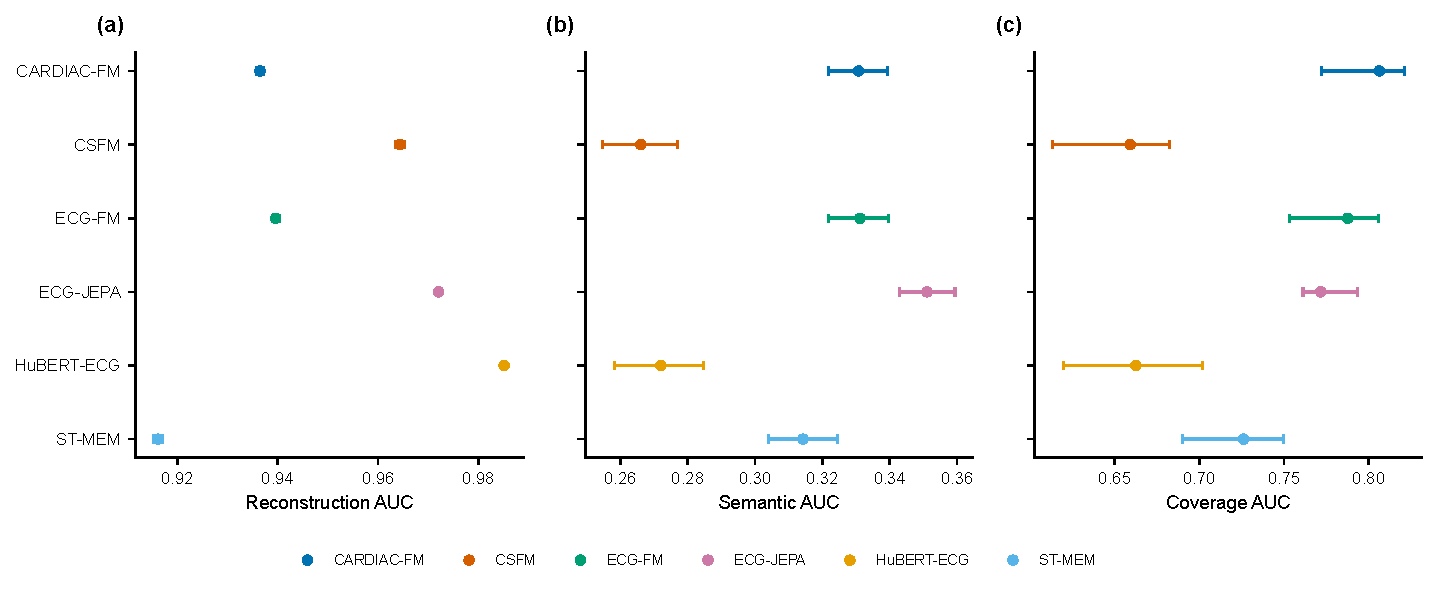
\includegraphics[width=0.86\textwidth]{figures/multiscale_patient_common_scale_auc.pdf}
  \caption{Metric-specific common-scale AUC estimates and paired patient-cluster intervals for (a) reconstruction, (b) single-coordinate clinical accessibility, and (c) concept coverage. A higher value is favorable within each panel, and the panels jointly characterize complementary dimensions of representation interpretability.}
  \Description{Three forest plots compare six ECG foundation models on reconstruction, single-coordinate clinical accessibility, and concept coverage after integrating the same five SAE scales.}
  \label{fig:profile-forest}
\end{figure*}

\subsection{External validation preserves metric-specific leaders}

We repeated the complete 450-cell multiscale SAE audit on a credentialed, patient-partitioned MIMIC-IV-ECG cohort; cohort construction and sensitivity analyses are detailed in Appendix~\ref{app:mimic-replication}. Table~\ref{tab:mimic-model-profiles} reports the held-out model profiles after integrating the same five-point expansion curve and averaging over the same five relative depths.

The replication reveals complementary leaders across interpretability dimensions. HuBERT-ECG has the highest reconstruction profile (0.990), whereas ECG-JEPA has the highest single-feature semantic alignment (0.324) and concept coverage (0.781). ECG-FM has the lowest dead-feature fraction (0.099) and the highest feature stability (0.378), while CSFM has the highest subspace stability (0.778). Together, reconstruction fidelity, local clinical accessibility, dictionary utilization, and cross-seed reproducibility provide a multidimensional comparison of the six models.

\subsection{A calibration ladder separates availability from localization}

Detailed calibration results are provided in Appendix Table~\ref{tab:accessibility-calibration}. The full SAE retains 79.9--87.4\% of dense-ridge mean $|r|$. Single SAE coordinates outperform the mean of 20 matched random dictionaries by 0.034--0.088 across every model's five depths, with 78.8--87.8\% concept--depth wins. These held-out results demonstrate consistent recovery of clinically aligned sparse structure by the learned SAE dictionaries across all six ECG FMs.

This calibration connects distributed concept availability with sparse localization. Full-code readouts quantify preserved clinical information, and single-coordinate readouts identify aligned sparse features across all six FMs. Together, these readouts establish the SAE profile as a common sparse instrument for comparing FMs.

The single-coordinate profile quantifies how strongly each clinical measurement is localized to one train-selected SAE coordinate and retained under held-out evaluation. Its 49-concept macro-average supports standardized model-level comparison, while the concept-level distribution reveals a substantial high-accessibility subset and resolves differences across waveform measurements. Together, these views provide both a common summary and concept-specific resolution of sparse clinical accessibility.

\subsection{Rank stability is itself a benchmark result}

Rank stability across SAE capacities is quantified over all ten pairs of common $E$ values. Reconstruction rank agreement has median Kendall $\tau=\MSReconMedianScaleTau$ and minimum $\tau=\MSReconMinScaleTau$; single-coordinate accessibility has median $\tau=\MSSemanticMedianScaleTau$ and minimum $\tau=\MSSemanticMinScaleTau$; coverage has median $\tau=\MSCoverageMedianScaleTau$ and minimum $\tau=\MSCoverageMinScaleTau$. Figure~\ref{fig:profile-forest} presents common-scale AUC as a capacity-robust summary, complemented by full curves for decisions tied to a particular SAE budget.

Rank agreement across $E$ directly tests whether an FM conclusion survives measurement capacity. The shared expansion grid provides a capacity-aware assessment of FM ordering under a common evaluation protocol. The current atlas also matches absolute width because every audited layer has $d=768$.

\begin{figure*}[t]
  \centering
  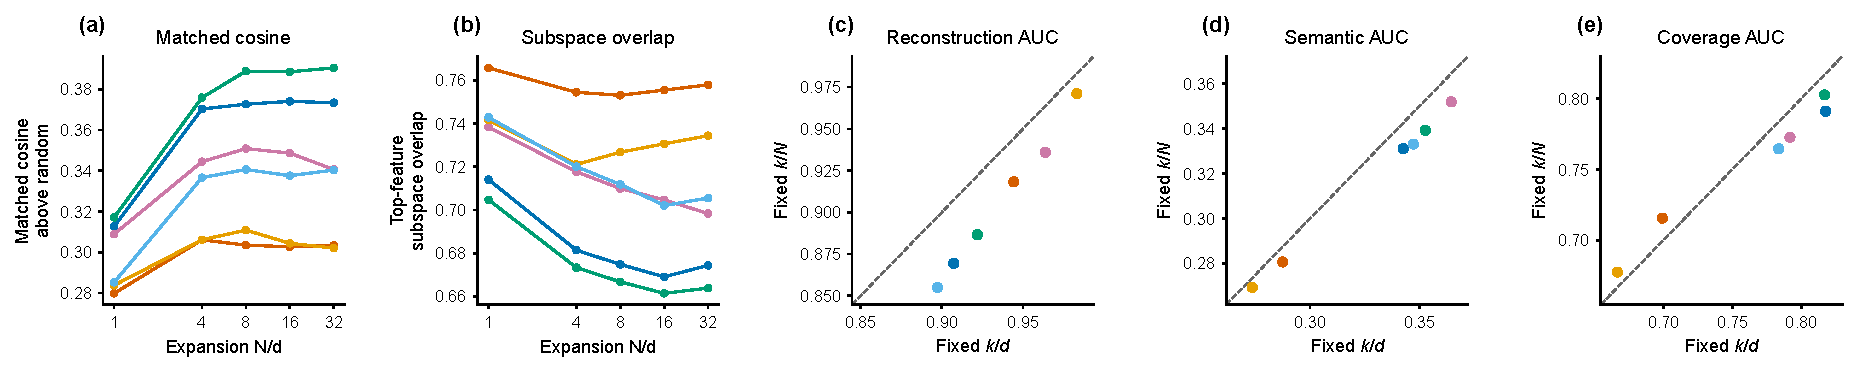
\includegraphics[width=\textwidth]{figures/multiscale_robustness_five_panel.pdf}
  
\includegraphics[width=0.74\textwidth]{figures/multiscale_robustness_legend.pdf}
  \caption{Robustness axes. (a) Cross-seed decoder matching above random and (b) selected-subspace overlap over common scale. Panels (c)--(e) show mid-depth common-scale AUC for reconstruction, clinical accessibility, and concept coverage under fixed $k/d$ and fixed $k/N$; the diagonal denotes unchanged profiles.}
  \Description{Five equal-size panels show feature stability curves and sparsity-sensitivity scatter plots for six models, with a separate legend below the panels.}
  \label{fig:stability-sensitivity}
\end{figure*}

\subsection{Feature identity and sparse fidelity are different axes}

Cross-seed matching asks whether a favorable fidelity or accessibility profile is implemented by reproducible decoder directions. The highest above-random matched-cosine AUC belongs to \MSStabilityTopModel{} (\MSStabilityTopAUC{}), whereas the highest selected-subspace overlap AUC belongs to \MSSubspaceTopModel{} (\MSSubspaceTopAUC{}). Figure~\ref{fig:stability-sensitivity}(a)--(b) shows how both quantities change over common scale. Joint reporting of stability, reconstruction, and single-coordinate clinical accessibility captures complementary representation properties.

Feature-level matching and selected-subspace overlap resolve two complementary forms of reproducibility across SAE seeds.

\subsection{Model ordering is tested under a second sparsity parameterization}

To isolate the effect of the active-code budget, we compare the primary fixed-$k/d$ arm with a preregistered fixed-$k/N$ arm at relative depth $q=0.5$. Because $d=768$, the primary arm uses $k=96$ at every $E$, whereas the sensitivity arm uses $k=\{12,48,96,192,384\}$ for $E=\{1,4,8,16,32\}$; dictionary widths, models, seeds, and training settings remain matched. Reconstruction ordering is highly stable across the two arms (median/minimum Kendall $\tau=1.00/0.87$), while accessibility ($0.73/0.60$) and coverage ($0.87/0.47$) respond more to the active budget, with the largest coverage reordering at $E=16$. Relative to fixed-$k/d$, fixed-$k/N$ changes common-scale AUC by $-0.012$ to $-0.042$ for reconstruction, $-0.004$ to $-0.014$ for accessibility, and $-0.027$ to $+0.016$ for coverage. At the shared $E=8$ anchor, both arms use $N=6144,k=96$, and independently trained cells differ by at most $0.0272$. Figure~\ref{fig:stability-sensitivity}(c)--(e) displays the corresponding model-level profiles.
